% ============================================================
%  Loop — AI Mock Interview Agent
%  Architecture Document
%
%  Compile: pdflatex ARCHITECTURE.tex (twice for refs)
%  Designed to compile cleanly on Overleaf with default packages.
% ============================================================
\documentclass[11pt,a4paper]{article}

% ---- Packages -------------------------------------------------
\usepackage[margin=1in,top=0.9in,bottom=0.9in]{geometry}
\usepackage[utf8]{inputenc}
\usepackage[T1]{fontenc}
\usepackage{lmodern}
\usepackage{amsmath}
\usepackage{tikz}
\usetikzlibrary{shapes.geometric, arrows.meta, positioning, calc, fit, backgrounds}
\usepackage{enumitem}
\usepackage{titlesec}
\usepackage{booktabs}
\usepackage{array}
\usepackage{caption}
\usepackage{hyperref}
\usepackage{fancyhdr}
\usepackage{parskip}

\hypersetup{
  colorlinks=false,
  pdfborder={0 0 0}
}

% ---- Header / footer ---------------------------------------
\pagestyle{fancy}
\fancyhf{}
\renewcommand{\headrulewidth}{0.4pt}
\renewcommand{\footrulewidth}{0pt}
\fancyhead[L]{\small Loop --- AI Mock Interview Agent}
\fancyhead[R]{\small Architecture Document}
\fancyfoot[C]{\small \thepage}

% ---- Section styling ----------------------------------------
\titleformat{\section}
  {\normalfont\large\bfseries}
  {\thesection.}{0.6em}{}
\titlespacing*{\section}{0pt}{14pt}{6pt}

\titleformat{\subsection}
  {\normalfont\normalsize\bfseries}
  {\thesubsection.}{0.5em}{}
\titlespacing*{\subsection}{0pt}{10pt}{4pt}

% ---- List styling -------------------------------------------
\setlist[itemize]{leftmargin=18pt, itemsep=3pt, topsep=3pt, parsep=0pt}
\setlist[enumerate]{leftmargin=20pt, itemsep=3pt, topsep=3pt, parsep=0pt}

% Caption styling
\captionsetup{font=small, labelfont=bf, skip=4pt}

% ============================================================
\begin{document}

% ============== TITLE BLOCK =================================
\begin{center}
  {\Large\bfseries Loop --- AI Mock Interview Agent}\\[4pt]
  {\large Architecture Document}\\[2pt]
  {\small Version 1.0 \quad $\cdot$ \quad May 2026}\\[6pt]
  \rule{0.8\textwidth}{0.4pt}
\end{center}

\vspace{6pt}

\noindent
\textbf{Abstract.} Loop is a multi-agent AI platform that parses a candidate's
résumé, infers realistic target roles with cited evidence, and conducts an
adaptive voice-driven mock interview while continuously analysing the
candidate's eye contact, posture, engagement, and stress signals from the
webcam feed. After the interview, the system synthesises a five-dimension
feedback report including STAR-method analysis of behavioural answers and a
specific coaching plan, then recommends live job postings ranked by semantic
match to the candidate's résumé. The platform was designed and built solo for
the IPHIPI Hackathon, with explainability and on-device inference as primary
design goals.

% ============== 1. PROBLEM SUMMARY ==========================
\section{Problem Summary}

Existing mock-interview tools fall into two categories, both inadequate.
Static-list tools cycle through hardcoded questions with no adaptation to the
candidate; large-language-model demos generate questions but provide no
visible reasoning, no feedback loop, and no signal that the system actually
learned anything about who it was interviewing.

Loop's design goal is to make the agent's reasoning \emph{visible} at every
step. When the system infers a target role, it cites the exact résumé bullets
that justified the inference. When the orchestrator adapts question
difficulty, it surfaces a one-line explanation (``Scored 0.42 --- dropping
difficulty to 2''). When the feedback synthesiser flags a weakness, it quotes
the literal phrase from the candidate's answer that triggered the flag. The
candidate finishes a session knowing not only their score but precisely why
they earned it and what to practice next.

\subsection{User Journey}

A complete session lasts eight to twelve minutes and follows seven stages:

\begin{enumerate}
  \item \textbf{Upload résumé.} The candidate uploads a PDF.
  \item \textbf{Role inference.} The system parses the résumé, extracts
        skills and experience, and proposes three target roles ranked by
        fit, each with cited evidence.
  \item \textbf{Pick interviewer.} The candidate selects a personality
        (warm coach, FAANG-style technical drill, or behavioural specialist).
  \item \textbf{Live interview.} The orchestrator generates questions
        dynamically, the candidate answers by voice, and the system scores
        each answer and adapts difficulty.
  \item \textbf{Multimodal observation.} Throughout the interview, the
        browser runs MediaPipe face and pose detection to track eye contact,
        posture, engagement, and stress.
  \item \textbf{Feedback synthesis.} On session end, the system produces a
        structured report combining the technical scoring, the multimodal
        observations, and STAR analysis of behavioural answers.
  \item \textbf{Job matching.} The candidate is shown a ranked list of live
        job postings drawn from a public API, each with a per-posting
        rationale for why it fits their profile.
\end{enumerate}

\vspace{4pt}

\begin{figure}[h]
\centering
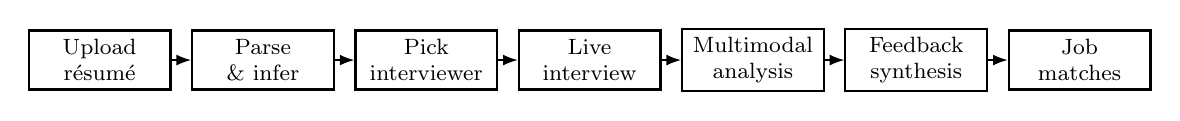
\begin{tikzpicture}[
    font=\footnotesize,
    node distance=2pt and 7pt,
    box/.style={
      draw=black, thick,
      minimum width=1.8cm, minimum height=0.75cm,
      align=center, inner sep=3pt
    },
    arr/.style={-Latex, thick, line width=0.5pt}
  ]
  \node[box]   (a) {Upload\\résumé};
  \node[box, right=of a]   (b) {Parse\\\& infer};
  \node[box, right=of b]   (c) {Pick\\interviewer};
  \node[box, right=of c]   (d) {Live\\interview};
  \node[box, right=of d]   (e) {Multimodal\\analysis};
  \node[box, right=of e]   (f) {Feedback\\synthesis};
  \node[box, right=of f]   (g) {Job\\matches};
  \draw[arr] (a) -- (b);
  \draw[arr] (b) -- (c);
  \draw[arr] (c) -- (d);
  \draw[arr] (d) -- (e);
  \draw[arr] (e) -- (f);
  \draw[arr] (f) -- (g);
\end{tikzpicture}
\caption{End-to-end user journey, executed in a single session.}
\end{figure}

% ============== 2. HIGH-LEVEL ARCHITECTURE ==================
\section{High-Level Architecture}

The system is organised into four layers: the browser client, a FastAPI
HTTP layer, a service layer that owns the core business logic, and external
or on-device dependencies. Figure~\ref{fig:arch} shows the full picture.

\begin{figure}[h]
\centering
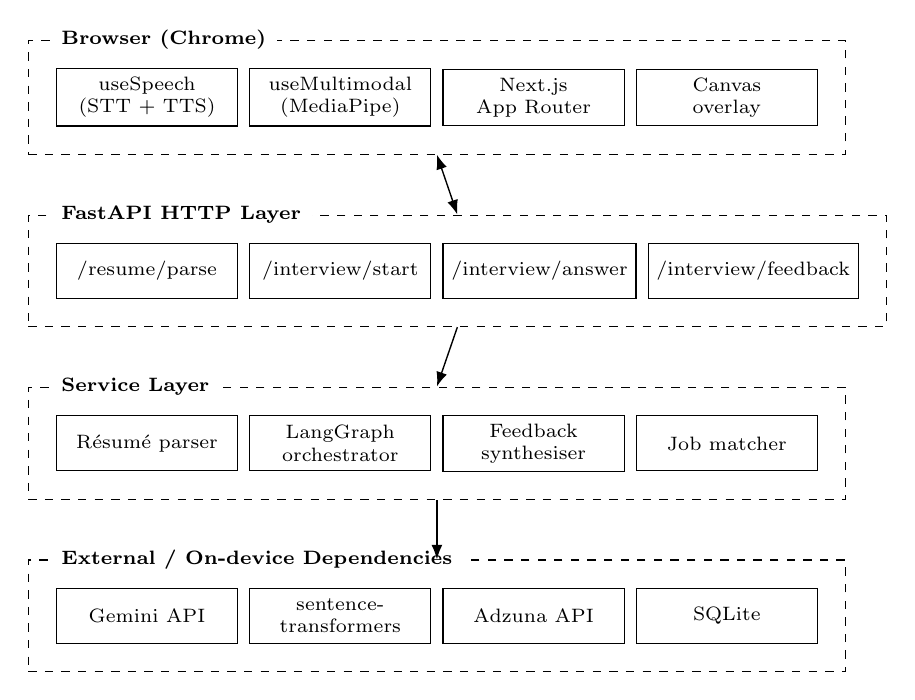
\begin{tikzpicture}[
    font=\scriptsize,
    box/.style={
      draw=black,
      minimum width=2.3cm, minimum height=0.7cm,
      align=center, inner sep=3pt
    },
    layer/.style={
      draw=black, dashed,
      inner xsep=10pt, inner ysep=10pt
    },
    arr/.style={-Latex, line width=0.5pt},
    bidir/.style={Latex-Latex, line width=0.5pt}
  ]

  % ===== Browser layer =====
  \node[box] (speech)  {useSpeech\\(STT + TTS)};
  \node[box, right=4pt of speech] (mm)  {useMultimodal\\(MediaPipe)};
  \node[box, right=4pt of mm] (ui)  {Next.js\\App Router};
  \node[box, right=4pt of ui] (cv)  {Canvas\\overlay};

  \begin{scope}[on background layer]
    \node[layer, fit=(speech)(mm)(ui)(cv)] (browser) {};
  \end{scope}
  \node[font=\bfseries\scriptsize, fill=white, inner xsep=4pt, inner ysep=1pt, anchor=west] at ([xshift=8pt,yshift=0pt]browser.north west) {Browser (Chrome)};

  % ===== API layer =====
  \node[box, below=42pt of speech] (resume)   {/resume/parse};
  \node[box, right=4pt of resume]  (start)    {/interview/start};
  \node[box, right=4pt of start]   (answer)   {/interview/answer};
  \node[box, right=4pt of answer]  (feedback) {/interview/feedback};

  \begin{scope}[on background layer]
    \node[layer, fit=(resume)(start)(answer)(feedback)] (api) {};
  \end{scope}
  \node[font=\bfseries\scriptsize, fill=white, inner xsep=4pt, inner ysep=1pt, anchor=west] at ([xshift=8pt,yshift=0pt]api.north west) {FastAPI HTTP Layer};

  % ===== Service layer =====
  \node[box, below=42pt of resume] (rparse) {Résumé parser};
  \node[box, right=4pt of rparse]  (orch)   {LangGraph\\orchestrator};
  \node[box, right=4pt of orch]    (synth)  {Feedback\\synthesiser};
  \node[box, right=4pt of synth]   (match)  {Job matcher};

  \begin{scope}[on background layer]
    \node[layer, fit=(rparse)(orch)(synth)(match)] (svc) {};
  \end{scope}
  \node[font=\bfseries\scriptsize, fill=white, inner xsep=4pt, inner ysep=1pt, anchor=west] at ([xshift=8pt,yshift=0pt]svc.north west) {Service Layer};

  % ===== External =====
  \node[box, below=42pt of rparse] (gem)  {Gemini API};
  \node[box, right=4pt of gem]     (st)   {sentence-\\transformers};
  \node[box, right=4pt of st]      (adz)  {Adzuna API};
  \node[box, right=4pt of adz]     (sql)  {SQLite};

  \begin{scope}[on background layer]
    \node[layer, fit=(gem)(st)(adz)(sql)] (ext) {};
  \end{scope}
  \node[font=\bfseries\scriptsize, fill=white, inner xsep=4pt, inner ysep=1pt, anchor=west] at ([xshift=8pt,yshift=0pt]ext.north west) {External / On-device Dependencies};

  % Connections
  \draw[bidir] (browser.south) -- (api.north);
  \draw[arr]   (api.south) -- (svc.north);
  \draw[arr]   (svc.south) -- (ext.north);
\end{tikzpicture}
\caption{System architecture across four layers. Approximately 60\,\% of
inference (speech, computer vision, embeddings) runs on the browser client.
Only question generation, answer scoring, and feedback synthesis require
calls to an external LLM.}
\label{fig:arch}
\end{figure}

\subsection{On-device Inference}

A deliberate design choice was to push as much inference as possible into
the browser. Speech-to-text and text-to-speech use the Web Speech API,
which is free and runs locally. Face and pose landmark detection use
MediaPipe Tasks JavaScript, which downloads small WebAssembly models once
and runs them on the CPU or GPU at approximately thirty frames per second.
Semantic embeddings for job matching use the
\texttt{sentence-transformers/all-MiniLM-L6-v2} model, an eighty-megabyte
download that runs locally on the FastAPI host. Only the
question generator, answer evaluator, and feedback synthesiser call out to
a remote large language model. This approach keeps the cost per session
near zero and avoids per-user API rate limits for the high-frequency
operations.

% ============== 3. AGENTIC LOOP =============================
\section{The Agentic Loop}

The core of the system is a LangGraph state machine that runs the
interview as a cyclic sequence of three nodes plus one conditional edge.
The state machine is shown in Figure~\ref{fig:graph}.

\begin{figure}[h]
\centering
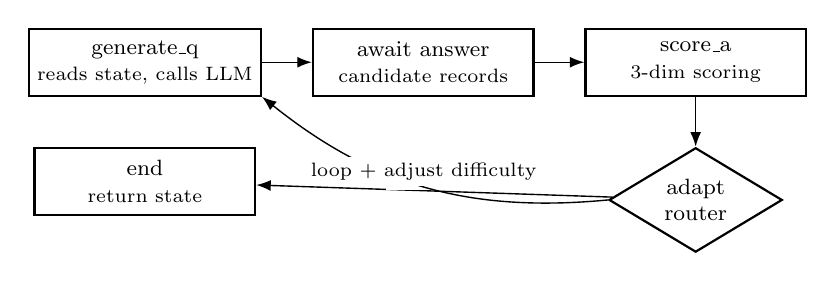
\begin{tikzpicture}[
    font=\footnotesize,
    node distance=10pt and 18pt,
    nd/.style={
      draw=black, thick,
      minimum width=2.8cm, minimum height=0.85cm,
      align=center, inner sep=3pt
    },
    decision/.style={
      diamond, draw=black, thick,
      minimum width=2.2cm, minimum height=0.8cm,
      align=center, inner sep=0pt
    },
    arr/.style={-Latex, line width=0.5pt},
    arrlbl/.style={font=\scriptsize, fill=white, inner sep=2pt}
  ]
  \node[nd]                            (gen)    {generate\_q\\\scriptsize reads state, calls LLM};
  \node[nd, right=of gen]              (await)  {await answer\\\scriptsize candidate records};
  \node[nd, right=of await]            (score)  {score\_a\\\scriptsize 3-dim scoring};
  \node[decision, below=18pt of score] (route)  {adapt\\router};
  \node[nd, below=18pt of gen]         (term)   {end\\\scriptsize return state};

  \draw[arr] (gen) -- (await);
  \draw[arr] (await) -- (score);
  \draw[arr] (score) -- (route);
  \draw[arr] (route) -- node[arrlbl, midway, above] {complete} (term);
  \draw[arr] (route.west) to[bend left=22] node[arrlbl, midway, above] {loop $+$ adjust difficulty} (gen.south east);
\end{tikzpicture}
\caption{LangGraph state machine. The orchestrator node \texttt{adapt\_router}
decides whether to terminate the interview or loop back with adjusted
difficulty. Its reasoning is written to the state as a one-line
natural-language explanation and surfaced live to the candidate.}
\label{fig:graph}
\end{figure}

\subsection{Routing Logic}

The adapt router applies the following rules after each answer is scored:

\begin{itemize}
  \item If the maximum number of questions has been reached, terminate.
  \item Otherwise, examine the score of the most recent answer:
  \begin{itemize}
    \item If the overall score is below 0.4, reduce difficulty by one level
          (minimum 1) and set a flag indicating the next question should
          open with an encouraging phrase.
    \item If the overall score is above 0.8, raise difficulty by one level
          (maximum 5).
    \item Otherwise, hold difficulty constant.
  \end{itemize}
  \item In all cases, write a one-line natural-language explanation of the
        decision to \texttt{state.last\_decision}.
\end{itemize}

The router's decision string is rendered live in the interview UI so the
candidate sees, in real time, why the next question changed in difficulty.
This is the project's primary demonstration of agentic behaviour as
distinct from a static question script.

\subsection{Interviewer Personalities}

The question generator's prompt is prepended with a personality directive
loaded from a separate module. Three personalities are supported:

\begin{itemize}
  \item \textbf{Mira} (warm coach). Patient, gives hints, restates questions
        when the candidate struggles. The default personality.
  \item \textbf{Marcus} (FAANG-style senior engineer). Cold, drilling, never
        validates effort. Presses on edge cases and scaling.
  \item \textbf{Priya} (behavioural specialist). Probes the how and why of
        decisions, explicitly requests STAR structure, asks for measurable
        outcomes.
\end{itemize}

Each personality also drives a distinct browser text-to-speech voice and a
distinct SVG avatar. The encouragement-on-low-score behaviour described
above is disabled for the Marcus personality so the candidate experiences
the cold style consistently.

% ============== 4. SCORING APPROACH =========================
\section{Scoring Approach}

Scoring runs in two stages. The hot path scores each answer as it is
submitted; the cold path synthesises the final report at session end. The
final report aggregates signals from three independent sources: LLM
semantic scoring of answer content, measured speech metrics from the
browser, and computer-vision-derived multimodal signals.

\subsection{Per-Answer Scoring (Hot Path)}

After each candidate answer, the \texttt{answer\_evaluator} agent returns
three sub-scores in the range $[0, 1]$:

\begin{itemize}
  \item \textbf{Correctness}: factual accuracy of technical claims.
  \item \textbf{Depth}: whether the answer probes the question at a
        sufficient level of detail.
  \item \textbf{Structure}: clarity of organisation, whether the answer
        follows a recognisable pattern such as STAR for behavioural
        questions.
\end{itemize}

These three sub-scores feed the adapt router and are stored on the session
state for use by the synthesiser.

\subsection{Speech and Visual Signals}

In parallel with the interview, two independent measurement layers run on
the browser:

\begin{itemize}
  \item \textbf{Speech metrics.} Filler-word frequency (counting ``um'',
        ``uh'', ``like'', ``you know'', and similar tokens), average words
        per answer, and speaking pace in words per minute. These are
        measured directly from the Web Speech API transcript and
        per-answer duration, not estimated by an LLM.
  \item \textbf{Visual metrics.} Eye contact (iris position relative to
        eye corners, combined with head pitch from nose-to-eye geometry),
        posture (shoulder symmetry and nose centring), engagement
        (composite of eye contact and head stability), and stress
        (composite of head movement variance, blink-rate anomaly, and eye
        avoidance). All four metrics are computed from MediaPipe face and
        pose landmarks, smoothed across a twelve-frame rolling window of
        approximately four hundred milliseconds.
\end{itemize}

The browser maintains per-session averages of all six metrics and submits
them with the feedback request.

\subsection{Final Report Synthesis (Cold Path)}

The feedback synthesiser is a single LLM call that receives the full
session transcript, the per-answer scores, and the multimodal averages,
and returns a structured JSON object containing the final five-dimension
report. The weighting is:

\vspace{4pt}
\begin{center}
\small
\begin{tabular}{lll}
\toprule
\textbf{Dimension} & \textbf{Weight} & \textbf{Primary signals} \\
\midrule
Technical correctness & 30\,\% & Per-answer correctness and depth \\
Communication clarity & 20\,\% & Filler-word frequency, words per answer, pace \\
Vocal confidence & 15\,\% & Hedging language, ``I don't know'' frequency, fillers \\
Engagement \& eye contact & 15\,\% & Eye-contact average, posture, head stability \\
Answer structure & 20\,\% & STAR analysis on behavioural answers \\
\bottomrule
\end{tabular}
\end{center}
\vspace{4pt}

The synthesiser is instructed to quote the candidate's literal words as
evidence in each improvement bullet, tag improvements by severity (low /
medium / high), produce a STAR breakdown for each behavioural answer with
per-component sub-scores, and generate exactly three coaching steps, each
under two hours of effort.

% ============== 5. KEY TRADE-OFFS ===========================
\section{Key Design Choices and Trade-offs}

Every architectural decision involved a deliberate trade-off. The most
significant ones are tabulated in Table~\ref{tab:tradeoffs}.

\begin{table}[!htbp]
\centering
\small
\caption{Key design trade-offs.}
\label{tab:tradeoffs}
\begin{tabular}{p{3.4cm} p{4.5cm} p{6cm}}
\toprule
\textbf{Decision} & \textbf{Chosen approach} & \textbf{Trade-off accepted} \\
\midrule
Computer vision & Browser MediaPipe with heuristic scoring & Free and scalable, but less accurate than a learned model. \\
\addlinespace
Speech to text & Web Speech API & Real-time and free, but lower accuracy on accented speech. \\
\addlinespace
Session storage & In-memory for live sessions; SQLite for completed sessions & Zero infrastructure; single-host only. \\
\addlinespace
Feedback synthesis & Single LLM call in JSON mode & Faster and atomic, but a single point of failure. \\
\addlinespace
Orchestrator & LangGraph state machine & Explicit nodes and easy to extend, but adds a dependency. \\
\addlinespace
Job feed & Adzuna public API & Terms-of-service compliant; limited to Adzuna's crawled feeds. \\
\addlinespace
Embeddings & sentence-transformers (local) & Zero API cost; lower ceiling than hosted models. \\
\addlinespace
LLM provider & Gemini 2.5 Flash (Lite for hot path, Pro for synthesis) & Generous free tier (1000 requests per day on Flash Lite) sufficient for demo workload. \\
\bottomrule
\end{tabular}
\end{table}

% ============== 6. LIMITATIONS ==============================
\section{Limitations, Assumptions, and Next Steps}

\subsection{Assumptions}

The system was designed under the following assumptions, all of which are
acceptable for the hackathon context but would need to be relaxed for a
production deployment:

\begin{itemize}
  \item A single user runs a single session at a time; there is no
        concurrent-interview support.
  \item Prompts and speech recognition are English-only. The Web Speech
        API supports more than one hundred languages, but the LLM prompts
        do not.
  \item Résumé PDFs are text-extractable. Scanned or image-only PDFs would
        require OCR preprocessing that is not currently implemented.
  \item The candidate uses Chrome with functioning webcam and microphone
        permissions granted.
\end{itemize}

\subsection{Known Limitations}

\begin{itemize}
  \item The computer-vision scoring is heuristic rather than learned.
        Accuracy degrades in poor lighting, with glasses, or with unusual
        camera angles.
  \item The LLM-derived ``confidence'' dimension overlaps partially with
        the measured filler-word count. Ideally the two sources would be
        cleanly separated.
  \item There is no real prosody model. Tone and pitch analysis are
        approximated by the LLM scoring the transcript text rather than
        by an actual acoustic-feature model.
  \item Sessions are persisted to SQLite for history, but the live session
        state is in-memory and is lost on backend restart mid-interview.
\end{itemize}

\subsection{Next Steps}

A six-month roadmap to take this from hackathon prototype to production
would address the limitations above and add several features that were
out of scope:

\begin{itemize}
  \item \textbf{Persistence layer.} Migrate session storage to Postgres
        with Redis for transient state. Add user accounts.
  \item \textbf{Trained computer-vision model.} Fine-tune a small
        classifier head on labelled interview footage to replace the
        heuristic eye-contact and posture scoring.
  \item \textbf{Whisper-based speech-to-text fallback.} Add a server-side
        Whisper deployment as an opt-in path for users with accents that
        Web Speech misses.
  \item \textbf{Acoustic prosody model.} Extract pitch variance, speech
        rate, and vocal energy with openSMILE or a small CNN. Feed these
        into the confidence dimension as a measured signal rather than an
        LLM estimate.
  \item \textbf{Recruiter mode.} Allow hiring managers to define custom
        assessments and have candidates take them asynchronously, with a
        structured rubric output. This is the natural revenue model for
        the platform.
  \item \textbf{Multi-language support.} Extend prompts and TTS voice
        selection to Hindi, Tamil, Spanish, and Mandarin via prompt
        templates.
  \item \textbf{Coding round.} Add a Pyodide-based browser Python execution
        sandbox with auto-graded test cases and LLM code review for
        technical roles.
\end{itemize}

\end{document}
